\documentclass[10pt,conference,compsocconf]{IEEEtran}

\usepackage{hyperref}
\usepackage{graphicx}	% For figure environment
\usepackage{enumerate}


\begin{document}
\title{Project 2 Machine Learning: Road Segmentation}

\author{
  Jakub Tarnawski, Damian Straszak, Kirtan Padh \\
  \textit{Department of Computer Science, EPFL, Switzerland}
}

\maketitle

\begin{abstract}
We propose a machine learning model which uses Convolutional Neural Networks(CNN) to extract roads from satellite images. We give a roadmap of how we arrived at our final model and describe it it detail, followed by the description of some advanced post processing steps using integer programming that we used to improve the accuracy. Our predictions based on this model achieve an f1 score of $91.704\%$ on the kaggle leaderboard.
\end{abstract}

\section{Introduction}
The problem statement we chose for the project is that given a satellite image taken from google maps, we need to classify each pixel as either road or background. We are given a training set of $100$ images of size $400 \times 400$ pixels, with each pixel classified appropriately. The testing set consists of $50$ images of size $608 \times 608$ pixels. This is a well studied problem in literature. Wang et al.\cite{wang16} give a comparison of the several different types of methods that have been used to tackle this problem.

Our methodology towards solving the problem is as follows.

\section{Methodology}
We are given two baseline methods for the project. One is a simple linear regression model and the other is a CNN with two convolutional layers and 2 pooling layers. We begin by trying simple classification techniques such as logistic regression and move on to more advanced techniques such as ADA boost and gradient boost and finally the baseline CNN given to us. Since we have access to a cluster on which we can train our model, we decide to first find a model which gives a reasonable good f1 score on the PC and then train it on the cluster.

Table 1\ref{baseline} summarizes the validation accuracies we get on trying increasingly complex classification models, but without doing a great amount of optimization on any of them. The f1 scores obtained are by doing a small grid search for each of the modes around the default parameters and cross-validating. 
\begin{figure}[h!]\label{baseline}
\center
\begin{tabular}{ l | c  }
  Model & f1 score $\pm$ standard deviation  \\
  \hline
  Logistic Regression (LR) & $65.9 \pm 2.311e^{-3}$  \\
  LR (polynomial basis) & $67.0 \pm 0.65$  \\
  ADA Boost & $26.37 \pm 1.26$ \\
  Gradient boost & $23.3 \pm 2.1$
\end{tabular}
\caption{Baseline comparison of classification models implemented and crossvalidated using scikit-learn}
\end{figure}
It seems that simple classification techniques are not easily able to achieve a good f1 score. Some of these models achieve an accuracy of around $75\%$, but not a good f1 score. So we try to see how well the CNN does. The validation scores for the given baseline CNN are shown in figure 2\ref{lr}. We used a patch size of $16$. We also tried patch sizes of $8$ and $4$, but the results were much worse, so w stick to $16$.
\begin{figure}\label{lr}
 \center
 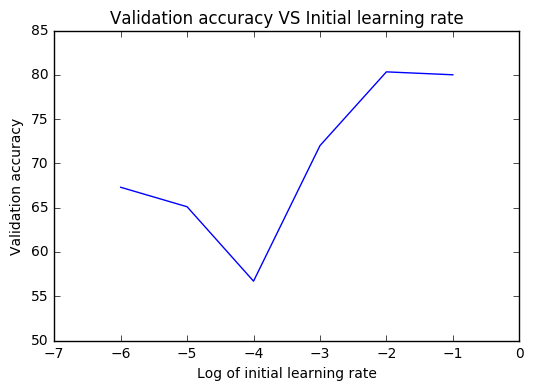
\includegraphics[scale=0.5]{lr.png}
 \caption{Validation accuracy VS Initial learning rate}
\end{figure}
We see that we already get an f1 score of $83.3\%$ when the learning rate is $0.01$, which is much better than the models we saw previously. So we try to fix the learning rate and train it on the cluster. We plot the loss curves in figure 3\ref{loss} for the different values of initial learning rates to get a better comparison along with the f1 score.  
\begin{figure}\label{loss}
 \center
 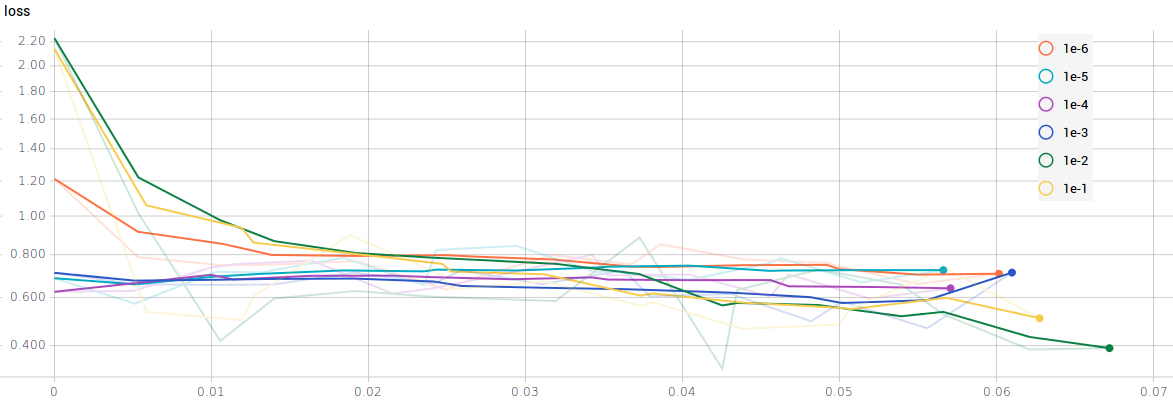
\includegraphics[scale=0.25]{loss_curves.png}
 \caption{The plot of the loss curves for each value of initial learning rate we tried. x-axis shows (number of iterations)/1000}
\end{figure}
We observe that while both $0.1$ and $0.01$ achieve a good f1 score, the loss curve for the value $0.01$ seems to be better as it is still decreasing with the increasing iteration, while the one for $0.1$ is starting to get stable. So we choose the initial learning rate to be $0.01$, and train the model on the cluster.

The only problem is that we do not have enough data as we have only a few training images. We solve this by generating several patches from a single image, as described in the next section, along with the details of the model.




\bibliographystyle{IEEEtran}
\bibliography{literature}

\end{document}
